\section{Timing and Hierarchical Coordination Operator between TFSM and Activity Languages}
\subsection{Overview}
	\begin{itemize}
		\item In this section, we use \bcool to specify two operators: \emph{startActivityWhenEnter} and \emph{AtomicActions}. Each operator captures a coordination pattern between the TFSM and Activity Language. 
		
		\item The \emph{startActivityWhenEnter} operator captures a hierarchical coordination pattern between the TFSM and fUML languages, unlike hierarchical coordination frameworks where the semantics is hidden, this operator explicitly specify how the hierarchical coordination is implemented. In our case, we chose the semantics in which entering a specific state of a TFSM model triggers the execution of a given fUML activity. When leaving a state, several semantic variation points may be chosen. The outgoing transitions from a state can be considered, for instance, as preemptive for the activity model (\ie firing a transition from a state to another preempts the internal activity). Alternatively, the transition can be considered as non-preemptive (\ie the states cannot be left before the associated activity finishes). In this example, we chose non-preemptive transitions. So that the state can be left only after the activity is finished. 
		
		\item In the \emph{AtomicActions} operator, we deal with the temporal aspects of the model coordination. The operator specifies how the time in the TFSM elapses during the execution of the activities that specify the on-entry action of a state. This coordination is also hierarchical, but in this case, only considers the timing aspects. In the TFSM language, each state machine has a \emph{localClock} used to measure the time (see Appendix~\ref{ap:languages}) while the fUML language is untimed. The local clock is a \emph{FSMClock}, which defines a \dse named \emph{ticks} whose occurrences represent a physical time increment. In the fUML language, the duration of activities can be represented as the time between the \dse \emph{startActivity} and \dse \emph{finishActivity} (see Appendix~\ref{ap:languages}). To coordinate the time, it is necessary to specify the number of \emph{ticks} of the local clock between the occurrence of the \dse \emph{startActivity} and \emph{finishActivity}. Thus the operator enforces the execution of the ``internal'' activity to be atomic with respect to the time in the TFSM model. As a result, there is no occurrence of the \dse ticks of the corresponding local clock during the execution of the activity.

		\item In the following, we define these operators in \bcool. Then, we use them to coordinate the heterogeneous model of a surveillance camera system (see Figure~\ref{fig:camerasystem}). We finish this section by studying the coordinated model.  


	\end{itemize}
	
	
	\subsection{Definition of the Coordination Operators}
	\begin{itemize}
		\item The \bcool specification is organized around two operators: \emph{startActivityWhenEnter} and \emph{AtomicActions}. 
		
		\begin{lstlisting}[language=bcool,
		caption={Hierarchical operator between TFSM and fUML languages},
		label={lst:bcoolStartActivityWhenEnter}, 
		basicstyle=\scriptsize\ttfamily, backgroundcolor=\color{LGrey}, numbers=left, xleftmargin=2pt]
		BCOoLSpec TFMSandActivityOperators
		ImportLib "facilities.moccml"
		ImportInterface "activitySemantics.ecl" as activity
		ImportInterface "TFSM.ecl" as tfsm
		Operator  StartActivityWhenEnter (activityStart : ad::startActivity , activityStop : ad::finishActivity, enterState : tfsm::entering, leaveState : tfsm::leaving)
		CorrespondenceMatching: when ((activityStart.name = activityStop.name ) and (enterState.name = leaveState.name) and (activityStart.name = enterState.onEnterAction.name));
		CoordinationRule: 
		LoopFromStartToFinishNonPeemptive (enterState, leaveState, activityStart, activityStop)
		end operator;
		\end{lstlisting}
		
		
		\item The \emph{startActivityWhenEnter}  (Listing~\ref{lst:bcoolStartActivityWhenEnter}) operator coordinates the action of entering into a state with the start of an activity so that when a state is entered, the execution of the activity is started synchronously. Then, the operator expresses that the leaving of the state follows the termination of the activity.   
		
		 \item Entering into a state is identified by the \textit{entering} \dse defined in the context of State. Instances of such \dse have to be coordinated with instances of the \textit{startActivity} \dse. Similarly, leaving a state is identified by \dse \textit{leaving} and finishing an activity is identified by \dse \textit{finishActivity}. 
		 
		 \item To identify pairs of events, we compare the \emph{onEnterAction} and the name of the activities (Listing~\ref{lst:bcoolStartActivityWhenEnter}: line 6). OnEnterAction is a method defined in the context of State (see Figure~\ref{fig:tfsmmm}). It specifies the name of the activity that the state represents. 
		  
		 
		 \item For the coordination rule, we have selected this semantics in which entering a state synchronously triggers the starting of an activity. Then, the coordination rule has to specify a causality between the finishing of the activity and the leaving of the state. 
		 
		 \item We rely on the event relation \emph{LoopFromStartToFinishNonPeemptive} (see Figures~\ref{fig:LoopFromStartToFinishNonPreemptive}). The event relation takes four events as argument: \emph{modeEnter}, \emph{modeLeave}, \emph{startActivity}  and \emph{finishActivity}. The \emph{modeEnter} and \emph{modeLeave} parameters are used to identify the entering and leaving of a state while the \emph{startActivity} and \emph{finishActivity} are used to identify the starting and finishing of an activity. 
		 
		 \item The FSM representation is based on two states: \emph{waitEnterState} and \emph{canLoop}. In the \emph{waitEnterState} state, the parameters can freely occur. When \emph{modeEnter} happens, the state \emph{canLoop} is reached and the activity can execute. More precisely, the events \emph{startActivity} and \emph{finishActivity} can occur thus making the activity execute in a loop. Then, only when the activity is finished and the state is left (\emph{modeLeve} occurs), the activity can leave the loop. This is represented by the transition from \emph{canLoop} to \emph{waitEnterState}.
		 
		 \item The use of this relation is our example results in a synchronization between \dse \emph{entering} and \emph{startActivity}, and causality relation between \dse \emph{leaving} and \emph{finishActivity}    
		 
		
		
			\begin{figure}
				\center
				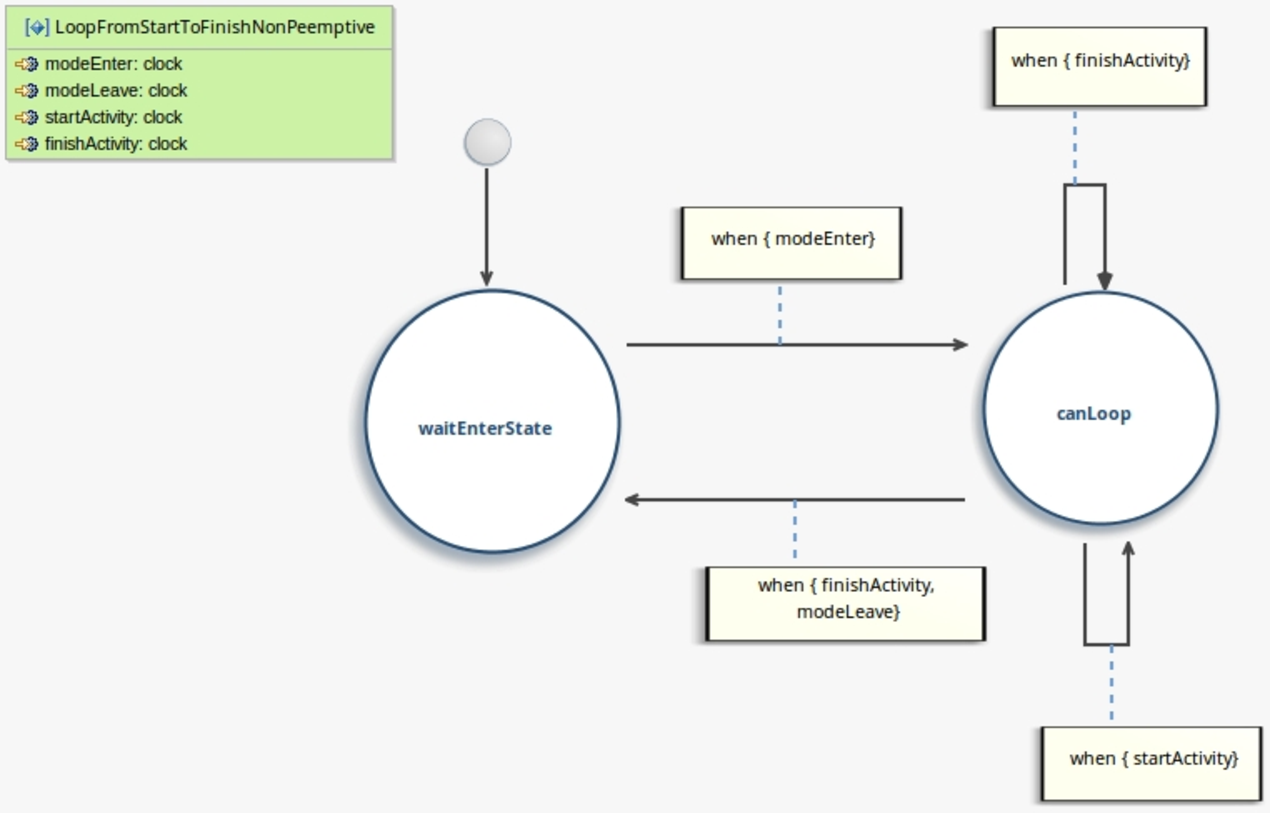
\includegraphics[scale=0.5]{examples/figs/LoopFromStartToFinishNonPreemptive.pdf}
				\caption{Graphical Representation of the Event Relation \emph{LoopFromStartToFinishNonPreemptive}}
				\label{fig:LoopFromStartToFinishNonPreemptive}
			\end{figure}
				
\begin{lstlisting}[language=bcool,
caption={Timing coordination operator between TFSM and fUML language},
label={lst:AtomicActions}, 
basicstyle=\scriptsize\ttfamily, backgroundcolor=\color{LGrey}, numbers=left, xleftmargin=2pt, firstnumber=11]
Operator  AtomicActions (activityStart : ad::startActivity , activityStop : ad::finishActivity, enterState : tfsm::entering, leaveState : tfsm::leaving, timeTicks : tfsm::ticks)
CorrespondenceMatching: when ((activityStart.name = activityStop.name ) and (activityStart.name = enterState.OnEnterAction.name ) and (enterState.owningFSM.localClock = timeTicks));
CoordinationRule: 
 AtomicExec (activityStart, activityStop, timeTicks)
end operator;
\end{lstlisting}
		
		\item The operator \emph{AtomicActions} is shown in Listing~\ref{lst:AtomicActions}. The operator must specify how time is consumed during the execution of the activities that are represented by states. The correspondence matching is similar than before. The only difference is we have to select instances of \dse ticks of the corresponding local clock. To do so, we use the selected instances of \dse entering to select instances of \dse ticks of the corresponding local clock. 
		
		\item In this example, we consider the execution of the activity is atomic. So that, during the execution of the activity, there are non ticks of the local clock. In other words, the local clock can only ticks only after the activity has finished its execution. To express such a coordination, we rely on the event relation \emph{AtomicExec}.  
		
		\item The event relation has three events as arguments: \emph{ticks}, \emph{startActivity} and \emph{finishActivity}. The FSM representation is based on two states: \emph{waitStartActivity} and \emph{waitfinishActivity}. In the state \emph{waitStartActivity}, the event ticks can freely happen. Conversaly, in the state waitfinishActivity, the ticks cannot occurs. The transition between these states are triggered by the events startAct and finishAct.  
		
		\item The use of this relation in our example makes the local clock only ticks when the activity is not being executed. 
		
		\begin{figure}
		  \center
		  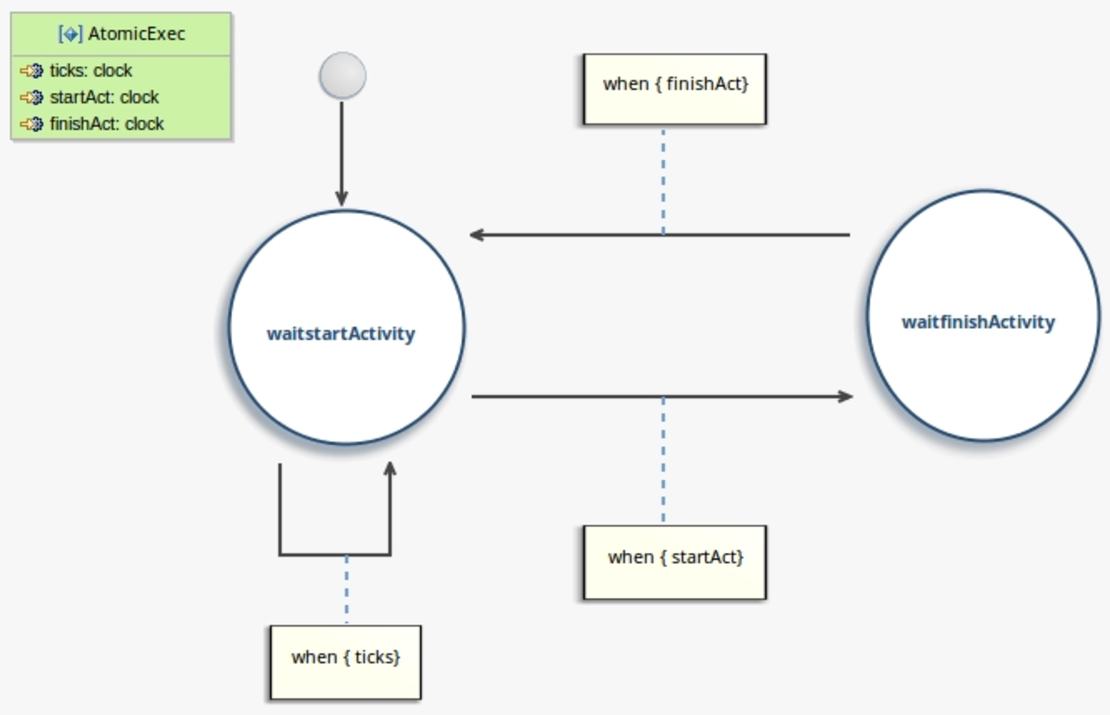
\includegraphics[scale=0.5]{examples/figs/AtomicExec.pdf}
		  \caption{Graphical Representation of the Event Relation AtomicExec}
		  \label{fig:LoopFromStartToFinishNonPreemptive}
		\end{figure}
					
		\item The use of the library to define domain specific relations has two major benefits. First, once defined in the library, event relations can be reused in various \bcool specifications. Second, by defining a dedicated event relation, we improve the readability and modularity of the \bcool specification.
	
	\end{itemize}

	\subsection{Use of the Operators in a Surveillance Camera System}
	
		\todo{to show a timing and state space exploration}
		
			\todo{to add vcd}
			
			
	In this section, we develop the heterogeneous model of a surveillance camera system (see Figure~\ref{fig:camerasystem}). To model different aspects of the system, we use the TFSM and the fUML languages. Then, we use the operators developed in the previous section to generate the coordination specification. 
	
	The video surveillance system is composed of a camera and a battery control. The camera takes pictures by using either the \emph{JPEG2000} or \emph{JPG} algorithm and is powered by a battery. When the battery is low, the battery control makes the camera use the \emph{JPG} algorithm, thus reducing the quality of the picture but also the energy consumption~\cite{encodingcomparison}. When the battery is high, the JPEG2000 algorithm is used instead. In Figure~\ref{fig:camerasystem}, the activity diagrams named \emph{BatteryControl} represents the simple algorithm implemented in the battery control. At the bottom of Figure~\ref{fig:camerasystem}, the TFSM named \emph{CameraControl} represents a partial view of the camera. When the TFSM model is in state \emph{BatteryHigh}, the JPEG2000 algorithm is used (specified by the activity diagram on the right of Figure~\ref{fig:camerasystem} named \emph{doJPEG2000}). When in state \emph{BatteryLow}, the encoding algorithm is replaced by a mere JPEG algorithm represented by an activity named \emph{doJPEG} (The activity is not shown for lack of space). The transition from one state to another is done when either the \emph{BatteryIsHigh} event or the \emph{BatteryIsLow} event occurs, depending on the current state.	 
	
	\begin{figure}
		\center
		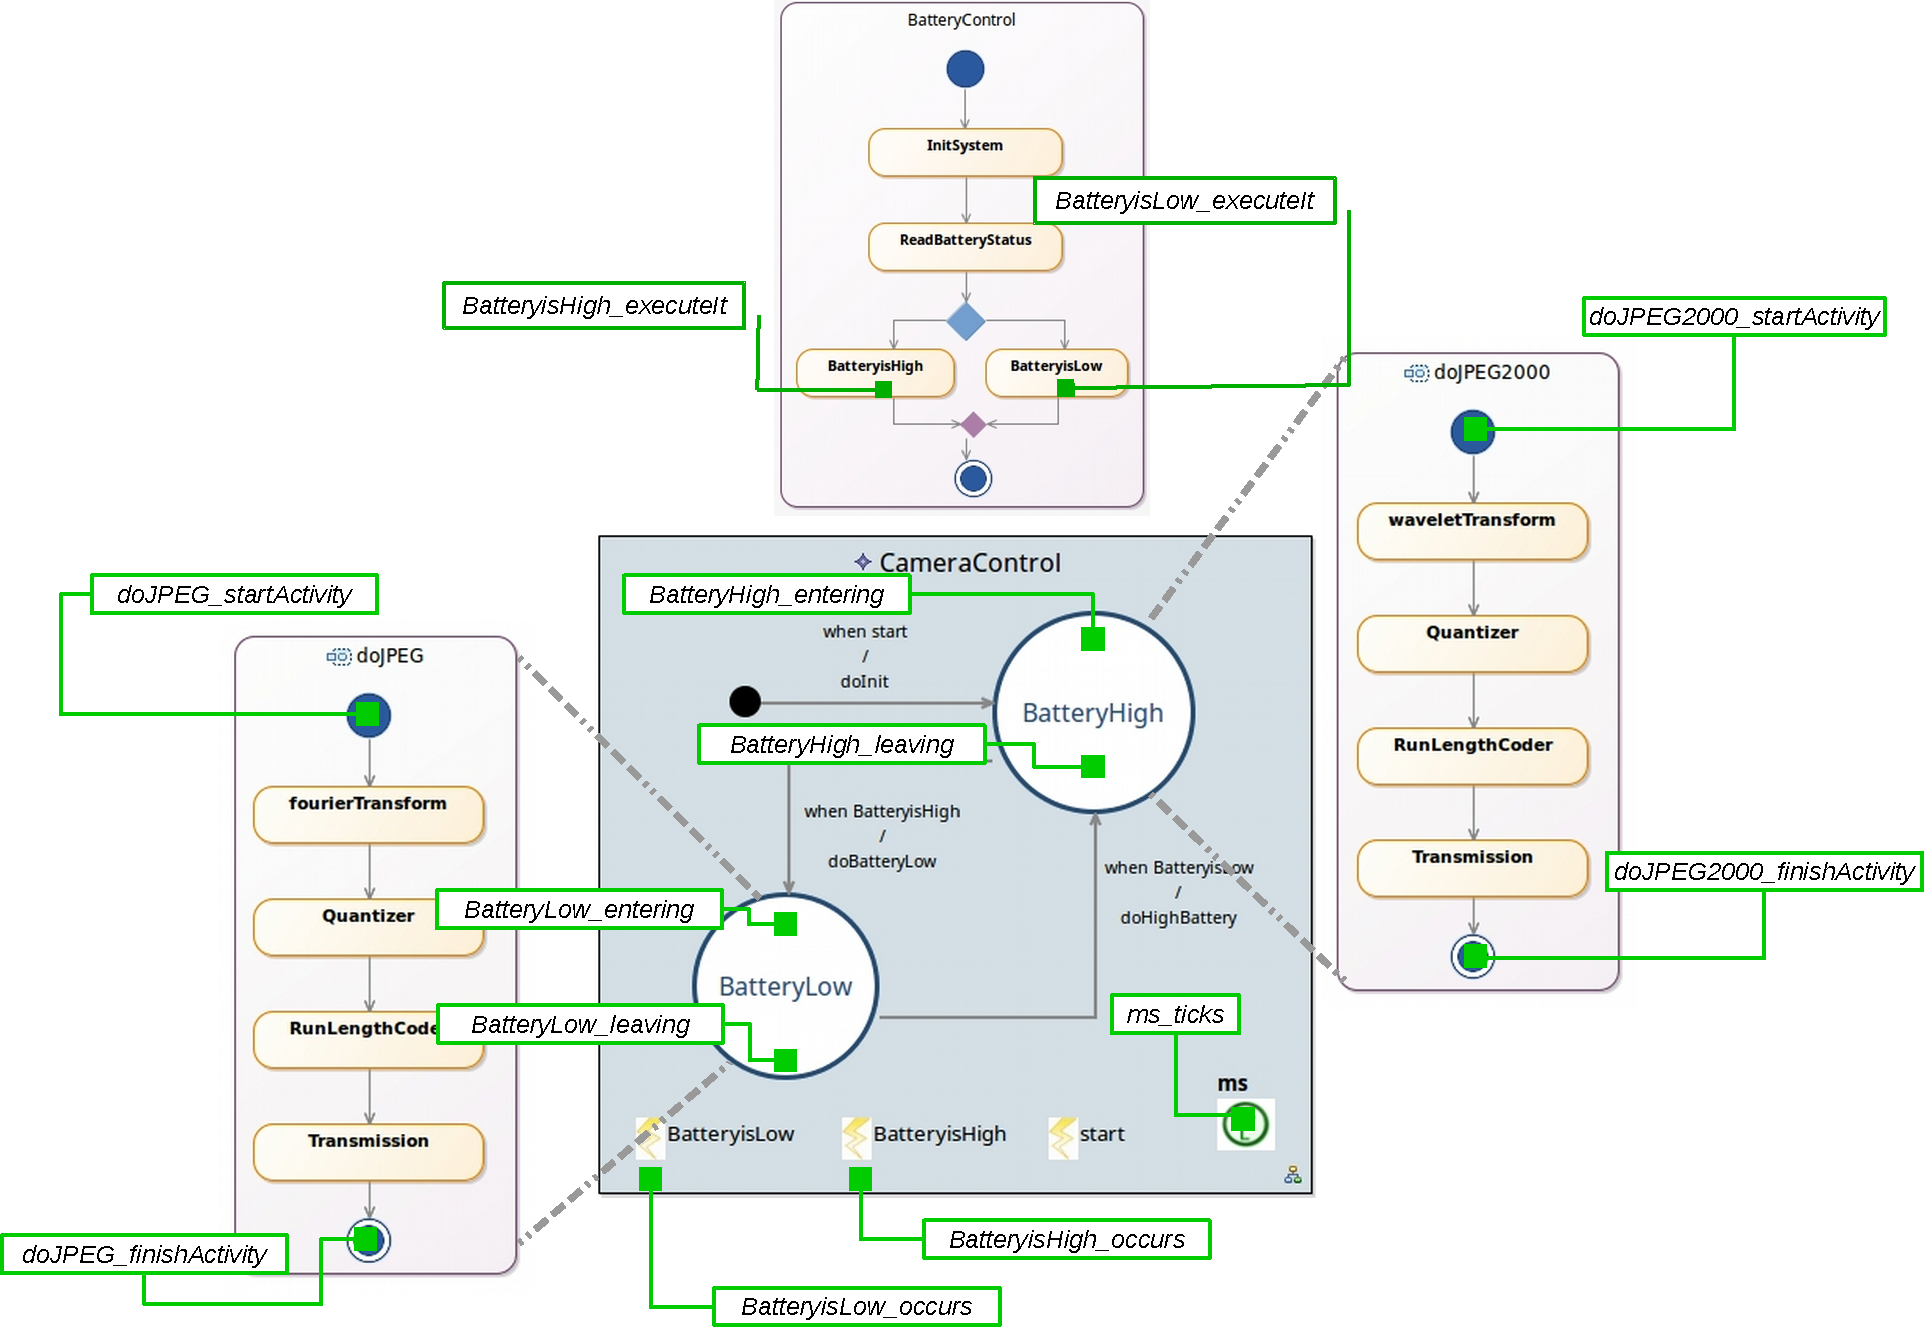
\includegraphics[width=.7\columnwidth]{examples/figs/picmodels.pdf}
		\caption{Hierarchical model of a surveillance camera system and a partial representation of the behavioral interface}
		\label{fig:camerasystem}
	\end{figure}
	
	To coordinate the models, we have to specify a timing and hierarchical coordination between the states of the TFSM CameraControl and the activities doJPEG and doJPEG2000. In addition, we have to synchronize the activity BatteryControl and the TFSM CameraControl by coordinating the corresponding Action and FSMEvent. Applying the four operators on these simple models, we generate the expected coordination specification. The coordination generated by using our approach corresponds to eight \ccsl relations.
	 
	In \bcool, the generated coordination specification conforms to the CCSL language. Since we are using a formal language, the integrator can execute and verify the coordination specification of the system.
	
	By using the language workbench presented in Section~\ref{section:bcoollengbench}, the coordination specification generated for the surveillance camera system can be executed and analysed. More precisely, we are able to execute the coordination specification by using TimeSquare, and to explore the state space. For lack of space we do not show the timing output of the execution of the surveillance camera system, however, the models together with a procedure to execute and verify them can be found in the companion web site.
	
	\subsection{Discussion}
	
	\begin{itemize}
		\item Discussion by relying on the criteria presented in evaluation.
		\item Semantics variation of the hierarchical coordination. 
		\item automatic generation of the coordination, eight relation.
		\item Verification and validation. 
	\end{itemize}